% Options for packages loaded elsewhere
\PassOptionsToPackage{unicode}{hyperref}
\PassOptionsToPackage{hyphens}{url}
%
\documentclass[
]{article}
\usepackage{amsmath,amssymb}
\usepackage{lmodern}
\usepackage{ifxetex,ifluatex}
\ifnum 0\ifxetex 1\fi\ifluatex 1\fi=0 % if pdftex
  \usepackage[T1]{fontenc}
  \usepackage[utf8]{inputenc}
  \usepackage{textcomp} % provide euro and other symbols
\else % if luatex or xetex
  \usepackage{unicode-math}
  \defaultfontfeatures{Scale=MatchLowercase}
  \defaultfontfeatures[\rmfamily]{Ligatures=TeX,Scale=1}
\fi
% Use upquote if available, for straight quotes in verbatim environments
\IfFileExists{upquote.sty}{\usepackage{upquote}}{}
\IfFileExists{microtype.sty}{% use microtype if available
  \usepackage[]{microtype}
  \UseMicrotypeSet[protrusion]{basicmath} % disable protrusion for tt fonts
}{}
\makeatletter
\@ifundefined{KOMAClassName}{% if non-KOMA class
  \IfFileExists{parskip.sty}{%
    \usepackage{parskip}
  }{% else
    \setlength{\parindent}{0pt}
    \setlength{\parskip}{6pt plus 2pt minus 1pt}}
}{% if KOMA class
  \KOMAoptions{parskip=half}}
\makeatother
\usepackage{xcolor}
\IfFileExists{xurl.sty}{\usepackage{xurl}}{} % add URL line breaks if available
\IfFileExists{bookmark.sty}{\usepackage{bookmark}}{\usepackage{hyperref}}
\hypersetup{
  pdftitle={Species ID Guide Template},
  pdfauthor={Meredith Miller},
  hidelinks,
  pdfcreator={LaTeX via pandoc}}
\urlstyle{same} % disable monospaced font for URLs
\usepackage[margin=1in]{geometry}
\usepackage{longtable,booktabs,array}
\usepackage{calc} % for calculating minipage widths
% Correct order of tables after \paragraph or \subparagraph
\usepackage{etoolbox}
\makeatletter
\patchcmd\longtable{\par}{\if@noskipsec\mbox{}\fi\par}{}{}
\makeatother
% Allow footnotes in longtable head/foot
\IfFileExists{footnotehyper.sty}{\usepackage{footnotehyper}}{\usepackage{footnote}}
\makesavenoteenv{longtable}
\usepackage{graphicx}
\makeatletter
\def\maxwidth{\ifdim\Gin@nat@width>\linewidth\linewidth\else\Gin@nat@width\fi}
\def\maxheight{\ifdim\Gin@nat@height>\textheight\textheight\else\Gin@nat@height\fi}
\makeatother
% Scale images if necessary, so that they will not overflow the page
% margins by default, and it is still possible to overwrite the defaults
% using explicit options in \includegraphics[width, height, ...]{}
\setkeys{Gin}{width=\maxwidth,height=\maxheight,keepaspectratio}
% Set default figure placement to htbp
\makeatletter
\def\fps@figure{htbp}
\makeatother
\setlength{\emergencystretch}{3em} % prevent overfull lines
\providecommand{\tightlist}{%
  \setlength{\itemsep}{0pt}\setlength{\parskip}{0pt}}
\setcounter{secnumdepth}{-\maxdimen} % remove section numbering
\usepackage[font=small,format=plain,labelfont=bf,up,textfont=normal,up,justification=justified,singlelinecheck=false]{caption}
\ifluatex
  \usepackage{selnolig}  % disable illegal ligatures
\fi

\title{Species ID Guide Template}
\author{Meredith Miller}
\date{10/18/2021}

\begin{document}
\maketitle

\newpage

\hypertarget{calliostoma-ligatum-blue-top-snail}{%
\section{\texorpdfstring{\emph{Calliostoma ligatum} (Blue top
snail)}{Calliostoma ligatum (Blue top snail)}}\label{calliostoma-ligatum-blue-top-snail}}

\hypertarget{description}{%
\subsection{Description}\label{description}}

\emph{Calliostoma ligatum}'s shells are cone-shaped with three distinct
convex whorls, and are generally 2.5 to 3 cm in diameter and 1.7 to 3 cm
tall (Tuskes 2019; Crowles 2004; Meschkat et al., 2013). ). The colour
of their unbeaded spiral ridges generally alternates between light
golden or tan and chocolate brown, although spirals can be white, grey,
black or red. If the shell is worn or damaged a distinctive blue inner
layer is visible, which can also be seen in the inner edge of empty
shells. The shell has a closed umbilicus, and its opening is rounded
with a pearly interior. The snail's foot has a distinctive bright orange
sole.

\emph{Calliostoma ligatum} is present from central Alaska to southern
California (Metschkat et al., 2013; Harbo 2011). It can be found
intertidally but also at depths of up to 30 meters in eel grass and kelp
beds, and rocky areas. Blue top snails are omnivorous, and although they
mainly consume \emph{Macrocystis} and other brown algae they also eat
diatoms, ascidians, sponges, bryozoans, and detritus (Crowles 2004;
Meschkat et al., 2013). Their main predators are sea stars and sunflower
stars, but, interestingly, they do not demonstrate antipredator
behaviour towards predatory snails (Hoffman, 1980). As broadcast
spawners, male \emph{Calliostoma ligatum} release sperm into the water
column, while eggs are released by females sheathed in mucous strands
that await fertilization (Holyvoak 1988). After fertilization, they
undergo several changes over 12 days to become planktonic larvae,
veligers, and then juvenile snails. They reach sexual maturity after 1
year. Blue top snails may be confused for Purple-ringed top snails
(\emph{Calliostoma annulatum}), but the beaded spirals on Purple-ringed
top snails are easily differentiated from the smooth spirals of Blue top
snails. Other snails in the area either do not have a similar top-like
shell morphology, or lack the distinguishable spirals and orange foot of
the top snails.

\hypertarget{identification-questions}{%
\subsection{Identification Questions}\label{identification-questions}}

\begin{enumerate}
\def\labelenumi{\arabic{enumi})}
\item
  Is the shell of the snail top shaped (not cone shaped) with three
  convex whorls?
\item
  Does the snail have a bright orange foot?
\item
  Are the spiral ridges on the snail's shell smoothed (not beaded)?
\end{enumerate}

\newpage

\hypertarget{figures}{%
\subsection{Figures}\label{figures}}

\begin{figure}

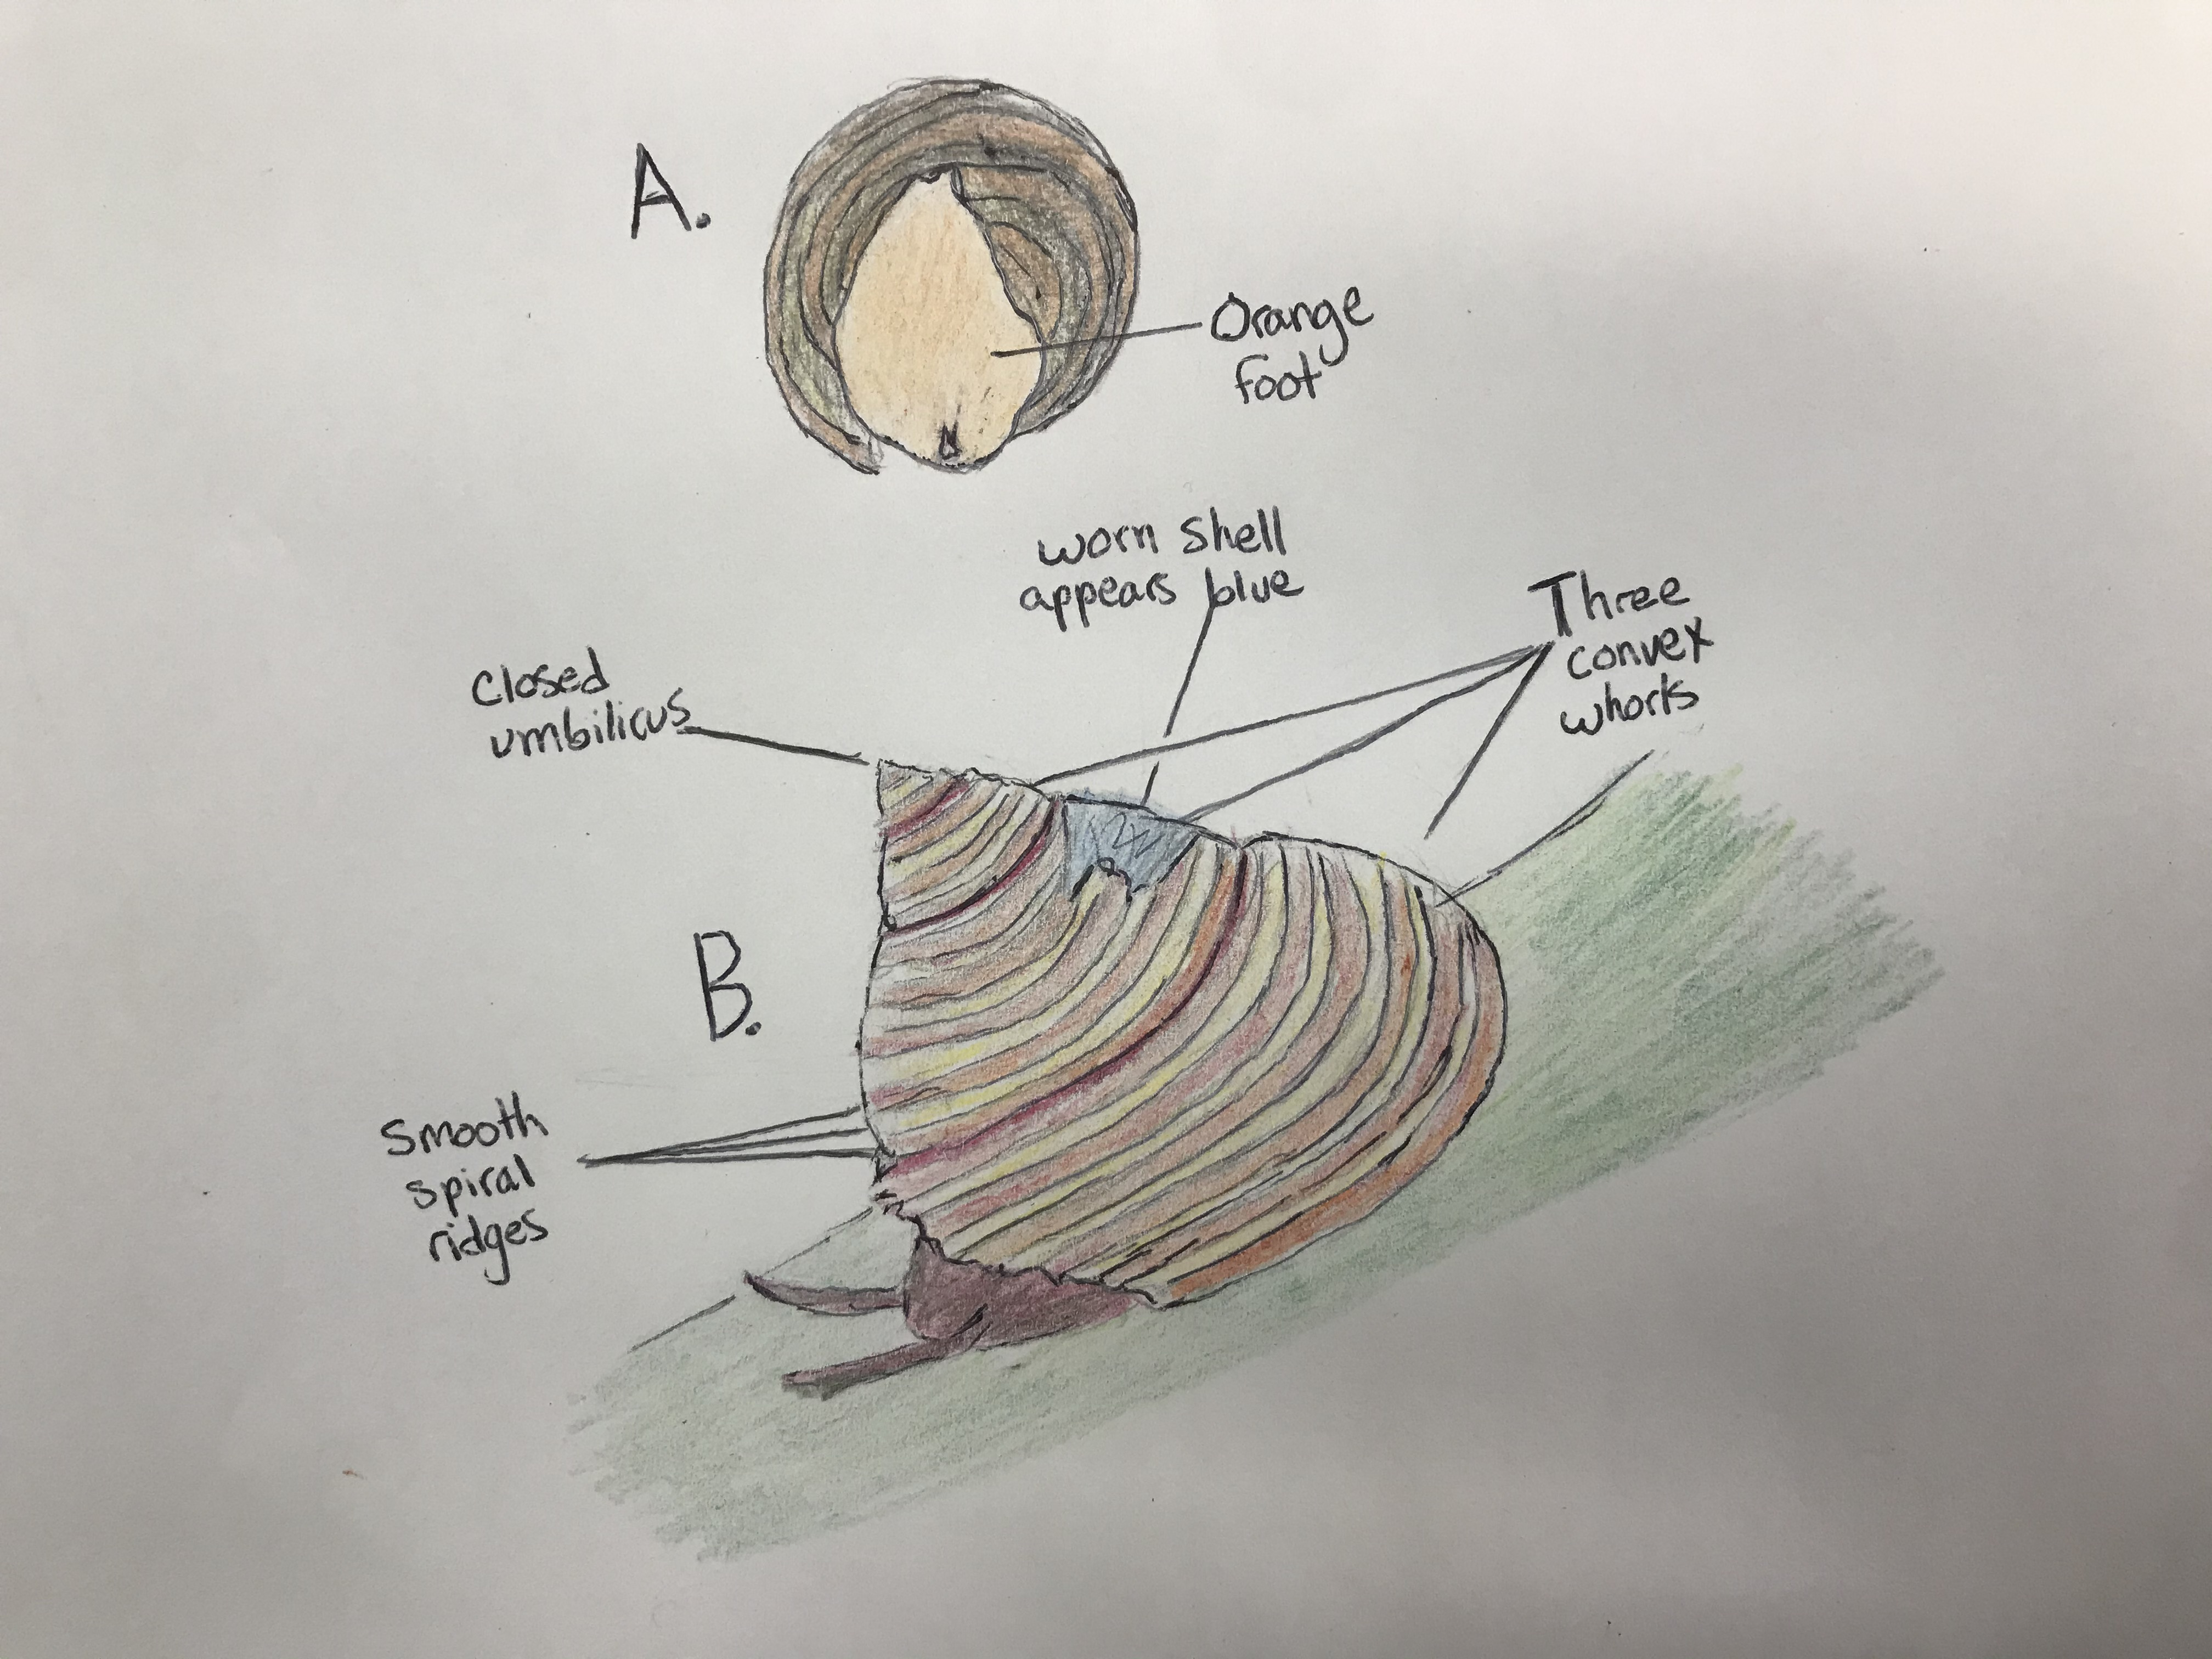
\includegraphics[width=0.5\linewidth,height=0.3\textheight]{/Users/mer/Github/species-id-guide-meredithyvr/images/Calliostoma_drawing} \hfill{}

\caption{Calliostoma ligatum positioned in ventral (A) lateral (B) views with important identifying characteristics labelled.}\label{fig:Calliostoma_drawing}
\end{figure}

\begin{figure}

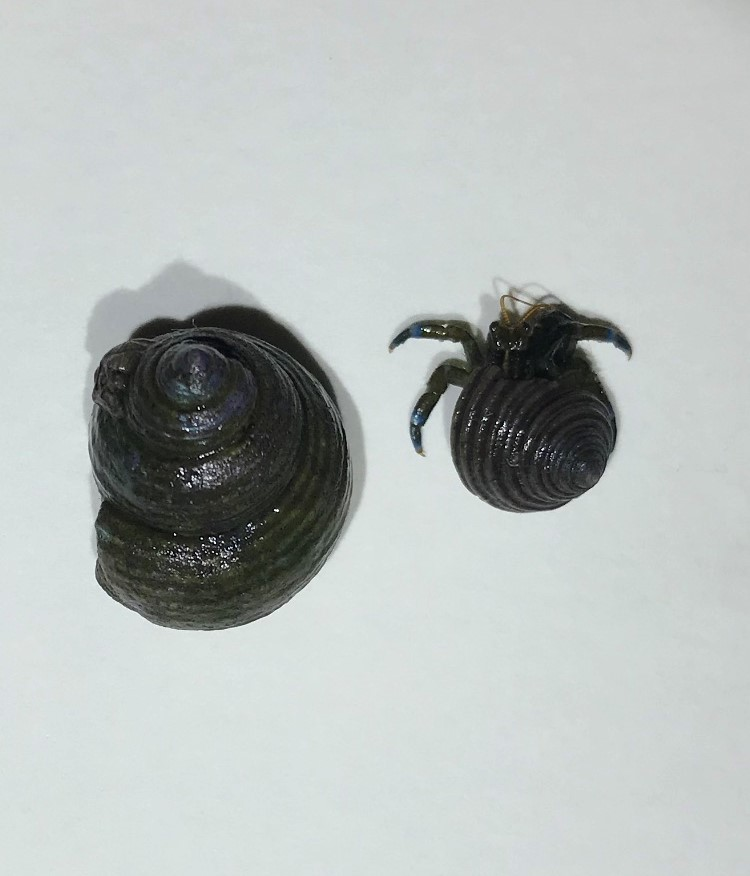
\includegraphics[width=0.5\linewidth,height=0.3\textheight]{/Users/mer/Github/species-id-guide-meredithyvr/images/Calliostoma_size} \hfill{}

\caption{Calliostoma ligatum shells (containing Hermit crabs) collected at Scott's Bay.}\label{fig:Calliostoma_size}
\end{figure}

\newpage

\hypertarget{nucella-lamellosa-frilledwrinkled-dogwinkle}{%
\section{\texorpdfstring{\emph{Nucella lamellosa} (Frilled/Wrinkled
Dogwinkle)}{Nucella lamellosa (Frilled/Wrinkled Dogwinkle)}}\label{nucella-lamellosa-frilledwrinkled-dogwinkle}}

\hypertarget{description-1}{%
\subsection{Description}\label{description-1}}

\emph{Nucella lamellosa's} shell can have very variable characteristics,
such as color and texture. Typically in solid colours, they can be light
brown, grey, to white, but can also have banding patterns (Harbo, 2011).
Some have even been observed in orange and purple colouring with
coloured bands. Their `frilled' name comes from their lamella, which
look like wrinkles or ruffles in the whelk's shell. A shell can have up
to 12 lamellae (Proudfoot \& Fretwell, 2015). Presence or absence of
frills in this species has been observed to vary with both wave and
predator (\emph{Cancer productus}) exposure. Typically, wave exposed
snails have smooth shells. Their shells are not `polished' looking and
are spirally coiled with 5-7 whorls (Bering et al.~2017). Overall, shell
shape is elongated into a point and can reach up to 80mm in height
(Proudfoot \& Fretwell, 2015). The shell mouth opening is ovate and the
lip of the shell is smooth and rounded with white coloring (or outside
shell colour) on the inside (Bering et al.~2017). Its operculum is
strongly spiraled and usually big enough to fully close the snail's
shell mouth opening, and it has a closed umbilicus (Bering et al.~2017).
Color, texture, thickness, coloured banding, and sometimes shape can
vary widely for this species (Proudfoot \& Fretwell, 2015). As there are
4 Nucella species in BC, this snail is commonly mistaken for its
relatives. Greyish or white \emph{N. lamellosa} can look a lot like
\emph{Nucella canaliculata}, however \emph{N. canaliculata} is typically
more streamlined in shape and doesn't have any frills on its shell
(Proudfoot \& Fretwell, 2015).

\emph{N. lamellosa's} range extends from Alaska (Aleutian Islands) to
California (central) (Proudfoot \& Fretwell, 2015; Harbo, 2011). This
range suggests Frilled Dogwinkles can live in a breadth of conditions,
but distributions suggest preference for cold temperate waters (Bering
et al.~2017). In terms of habitat preferences, these snails inhabit the
rocky intertidal, specifically mid to low zones but can be in shallow
subtidal locations as well (Proudfoot \& Fretwell, 2015; Harbo, 2011).
The Frilled Dogwinkle inhabits rocky crevices, rock faces, as well as
barnacle and mussel beds. Frilled Dogwinkles are predatory and feed on
mussels and acorn barnacles (among other mollusks) by drilling into them
with their radula and using a siphon that penetrates the prey's shell to
feed on internal tissues (Carefoot, 2021). Mating occurs in winter and
spring. Sexually mature (\textgreater4yrs old) snails aggregate to breed
with a group at their original hatching site (Bering et al.~2017).
Females spawn eggs after 20 months and baby snails hatch from them after
140 days. Eggs are contained in capsules that protect them from factors
such as salinity stress. Eggs (``sea oats'') are pale yellow and shaped
like \textasciitilde10mm vases, they can be observed on rocks in
clusters (Bering et al.~2017).

\hypertarget{questions}{%
\subsection{Questions}\label{questions}}

\begin{enumerate}
\def\labelenumi{\arabic{enumi})}
\item
  Does the snail have 5-7 whorls, with the last whorl being the largest
  by far?
\item
  Does it have an oval aperture that is around half the length of the
  shell?
\item
  Is the lip thick, rounded, and smooth, with white or the shell's outer
  color showing through?
\end{enumerate}

\newpage

\hypertarget{figures-1}{%
\subsection{Figures}\label{figures-1}}

\begin{figure}

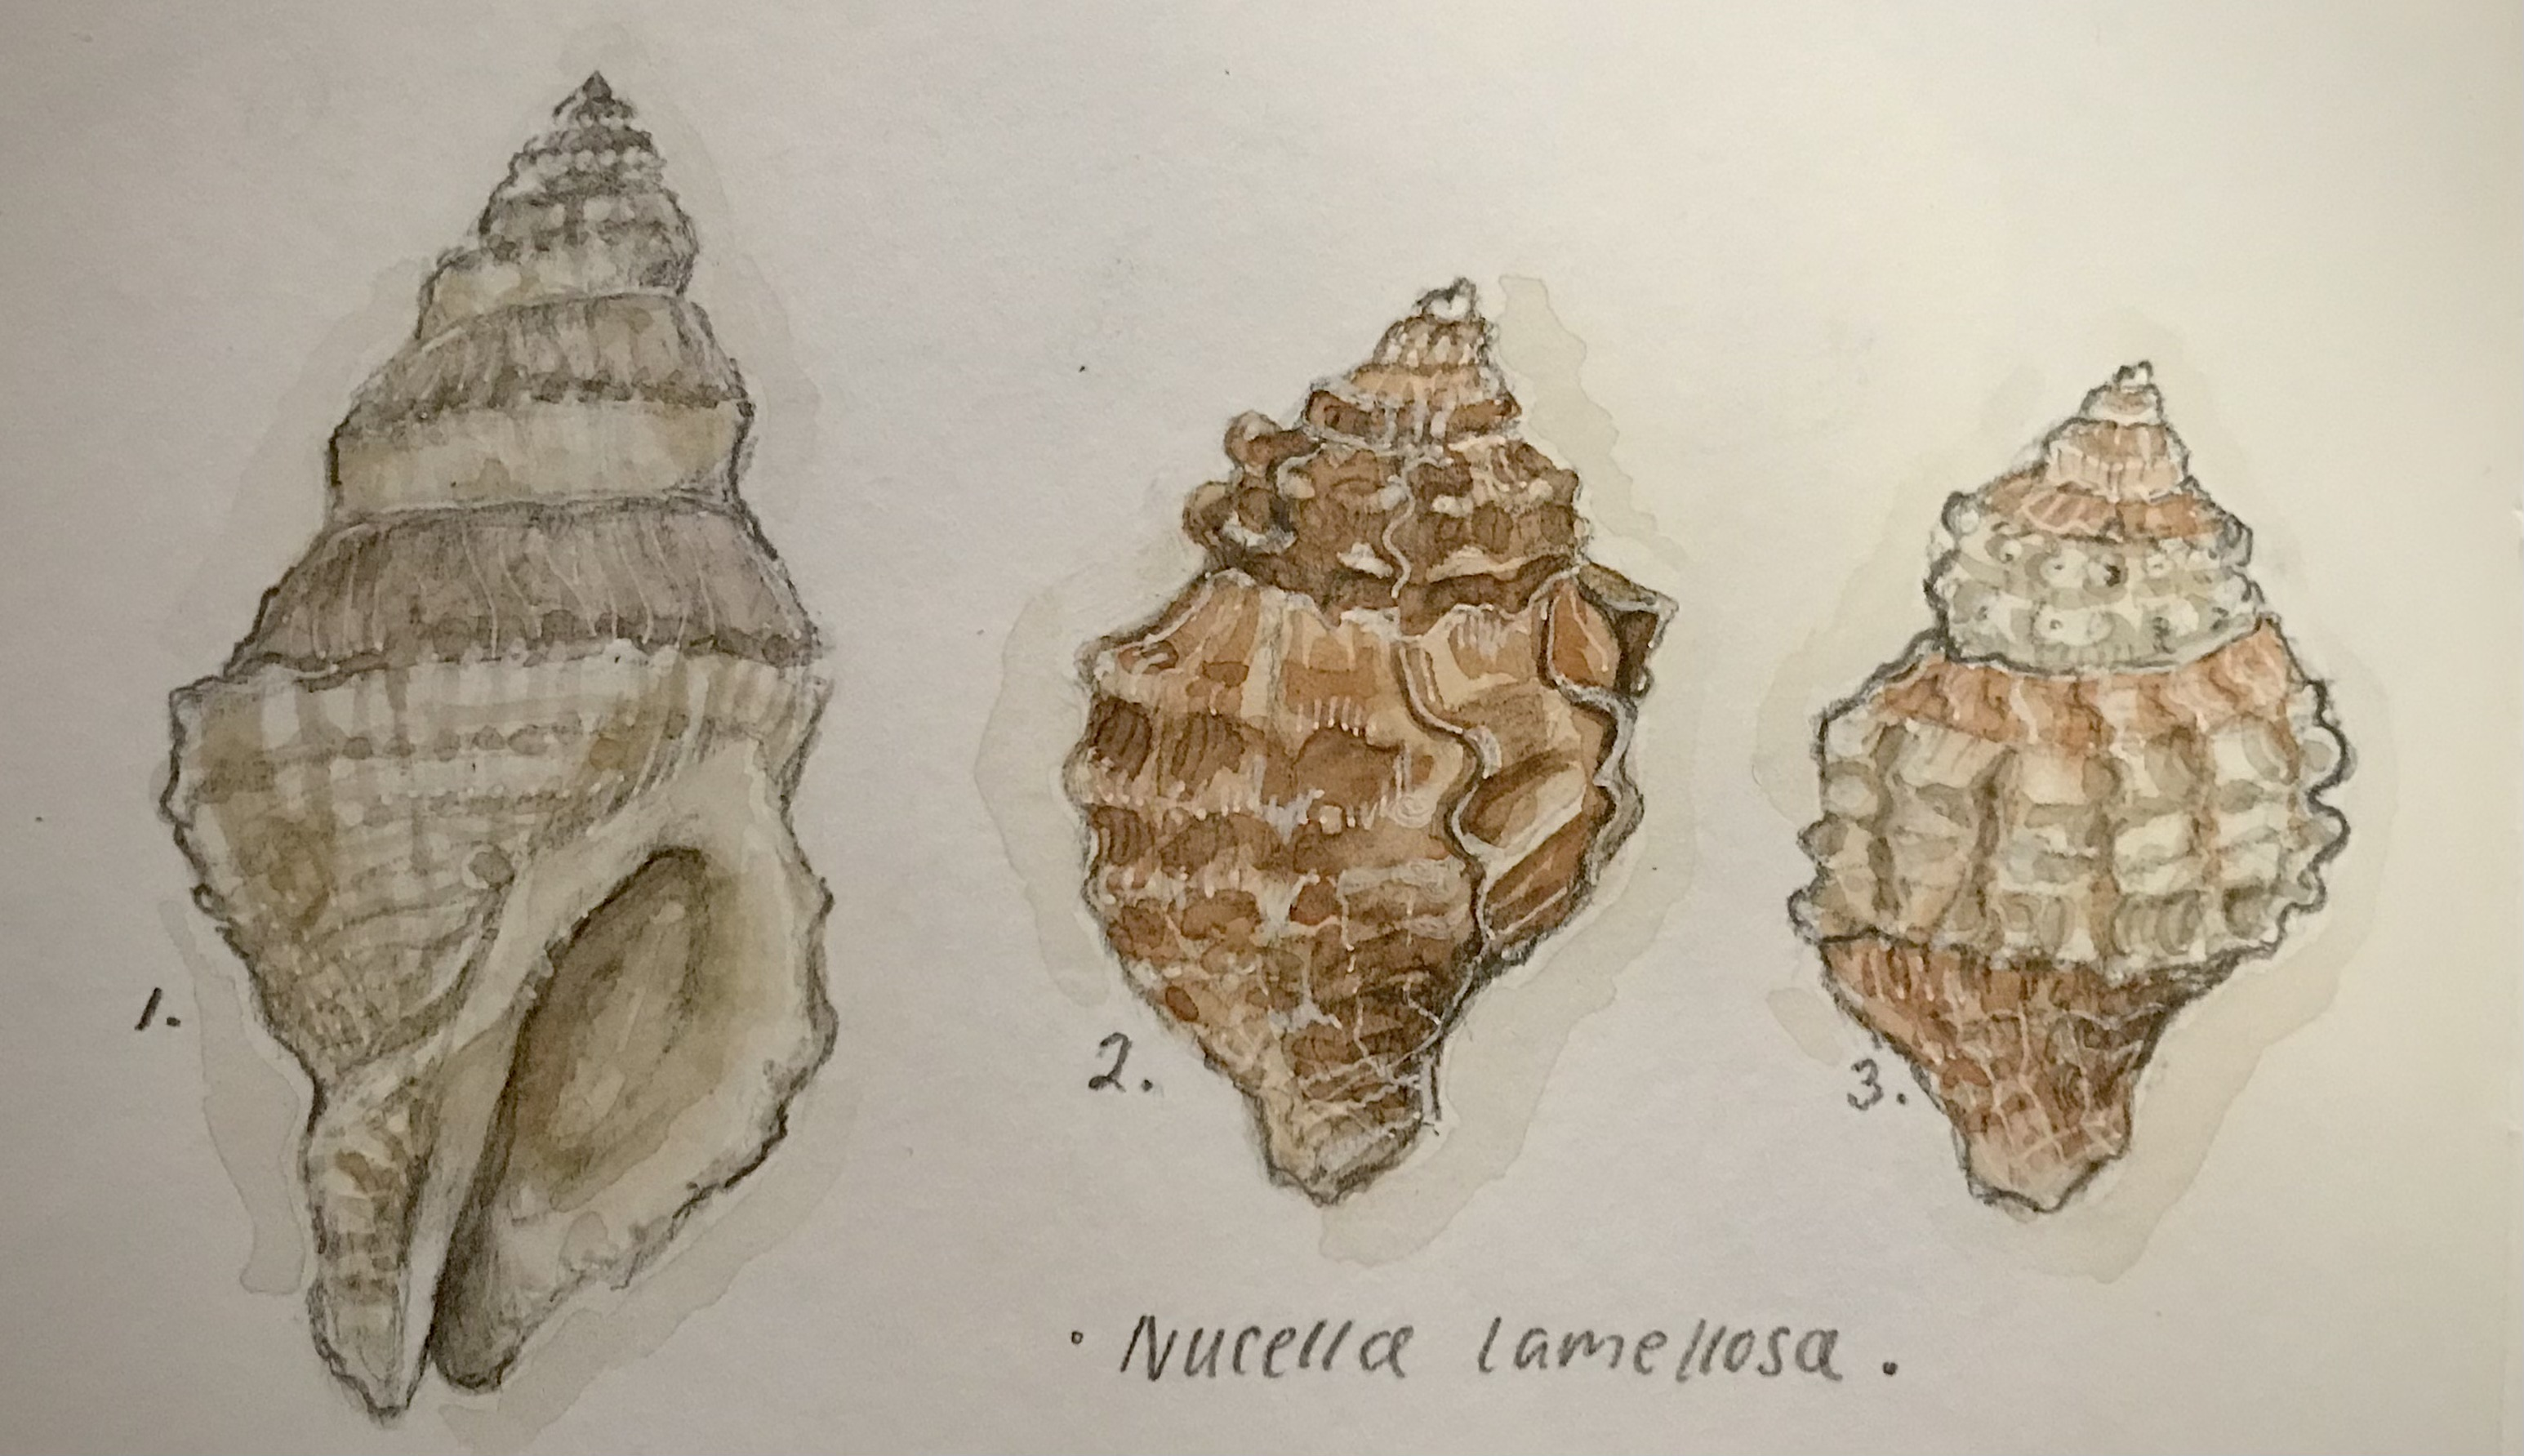
\includegraphics[width=0.5\linewidth,height=0.3\textheight]{/Users/mer/Github/species-id-guide-meredithyvr/images/nucella_lamellosa} \hfill{}

\caption{A drawn diagram of *Nucella lamellosa* (L.Wall). These drawings show the morphological variety in shell colours, textures, and banding. 1) shows underside of the snail, highlighting the oval aperture. 2) shows an upright view of the snail, showing frills, five distinct whorls, and brown colouring. 3) shows a banding colour pattern and less frilly surface.}\label{fig:Nucella_lamellosa}
\end{figure}

\begin{figure}

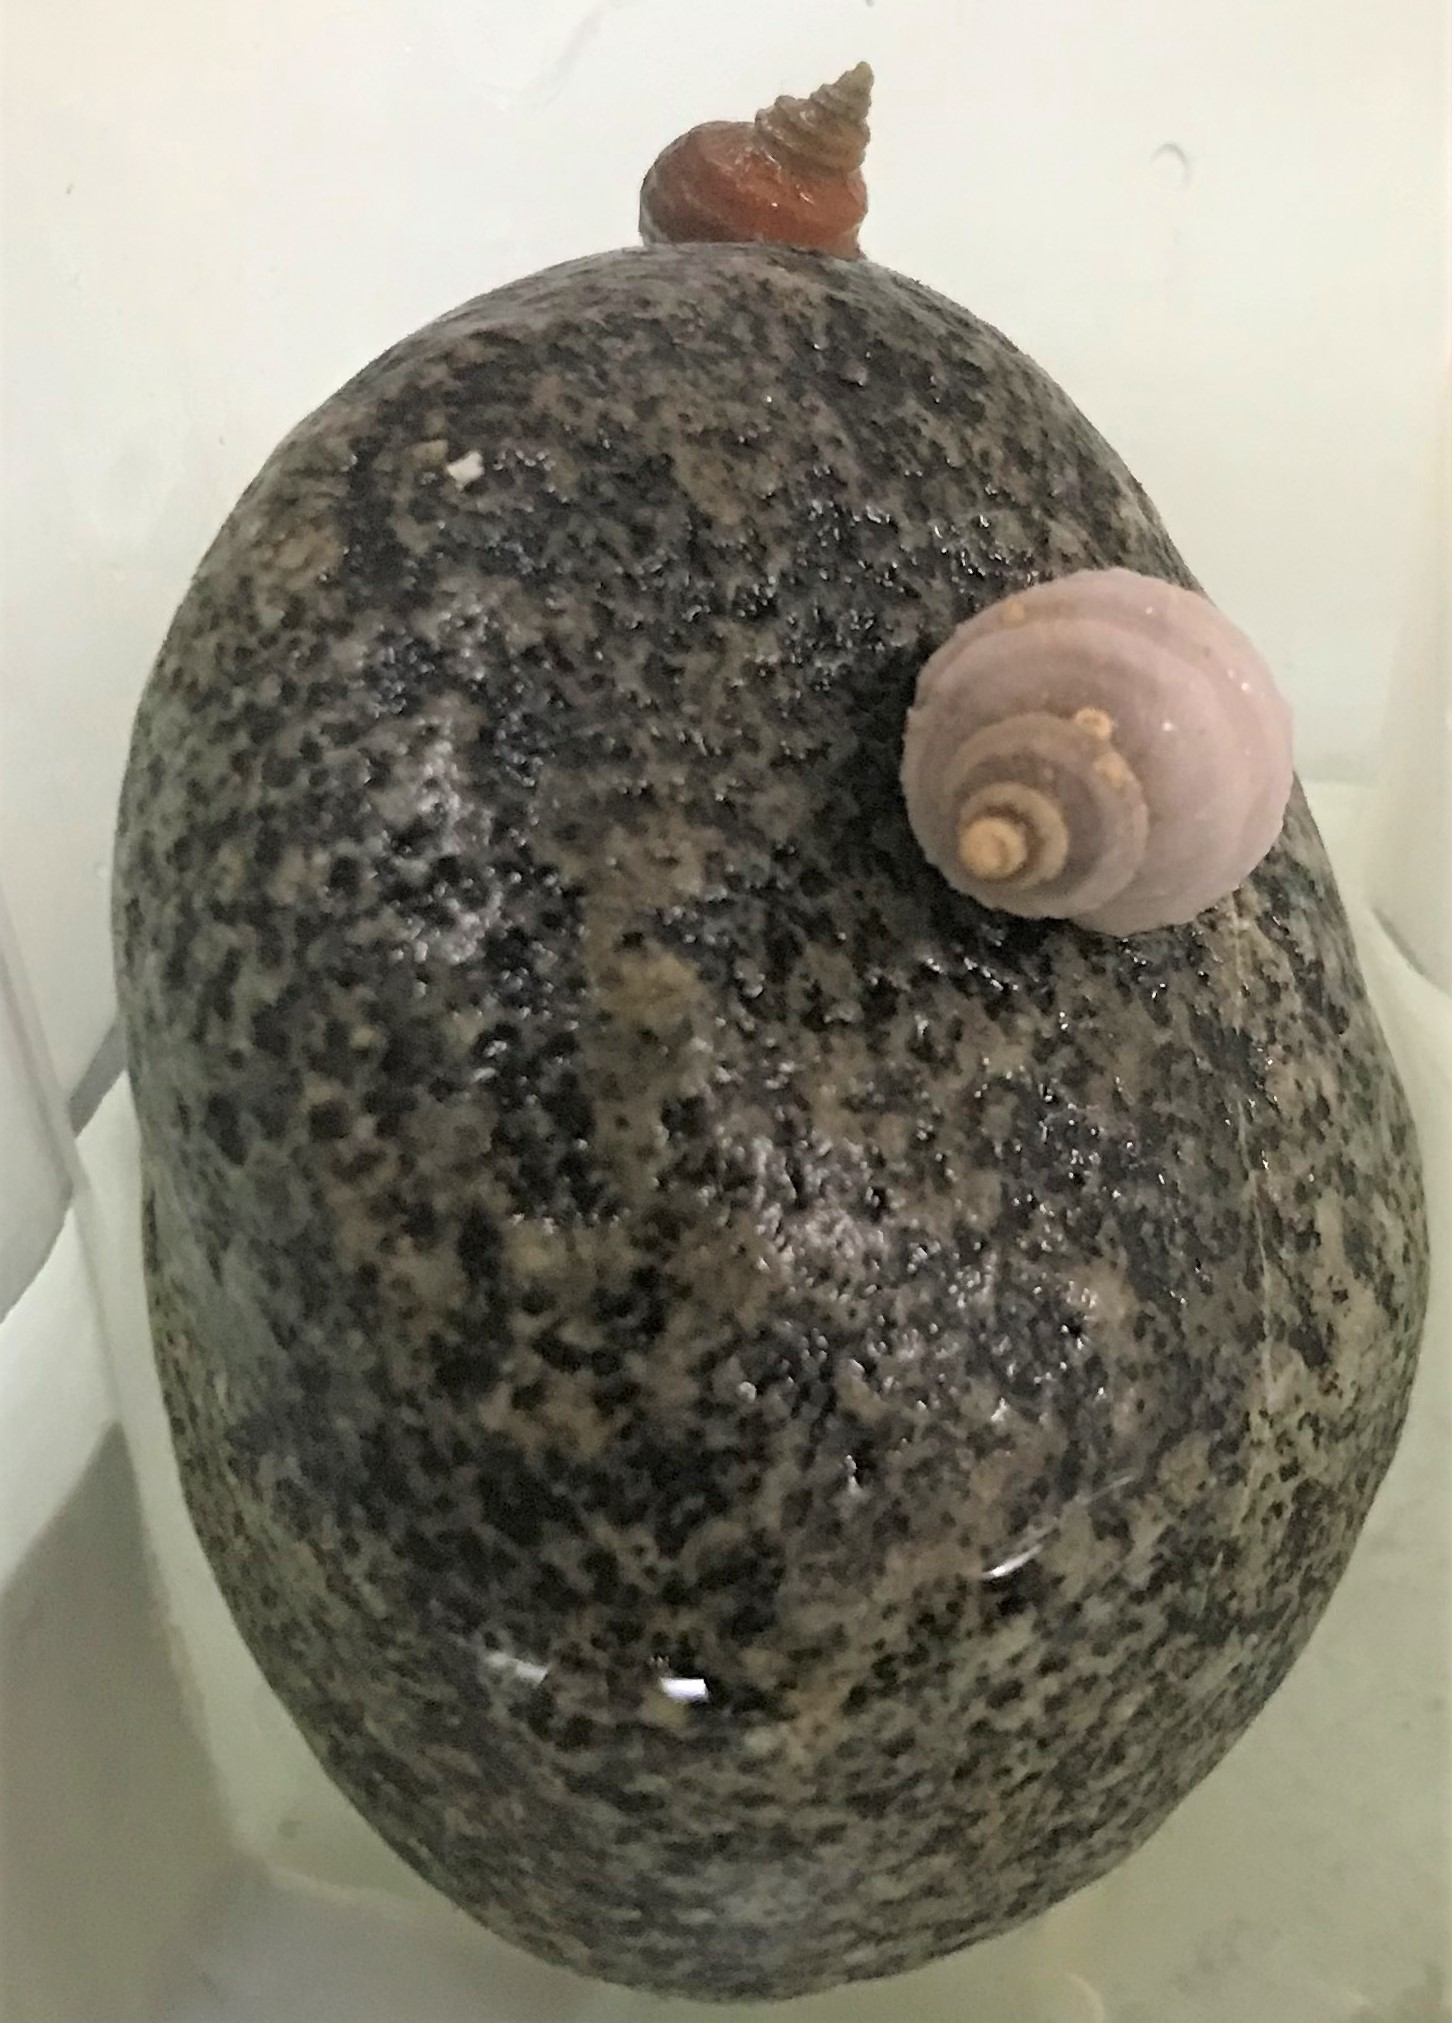
\includegraphics[width=0.5\linewidth,height=0.3\textheight]{/Users/mer/Github/species-id-guide-meredithyvr/images/snailonrock} \hfill{}

\caption{Photos showing two varieties of *N. lamellosa* snails collected from Scotts Bay in Bamfield, BC on October 15th 2021 (L.Wall). This highlights the variation in snail color and size, with smooth shell morphology suggesting plastic suitability to their wave-exposed habitat. }\label{fig:SnailonRock}
\end{figure}

\newpage

\hypertarget{tegula-funebralis-black-tegulablack-turban-snail}{%
\section{\texorpdfstring{\emph{Tegula funebralis} (Black Tegula/Black
Turban
Snail)}{Tegula funebralis (Black Tegula/Black Turban Snail)}}\label{tegula-funebralis-black-tegulablack-turban-snail}}

\hypertarget{description-2}{%
\subsection{Description}\label{description-2}}

The \emph{Tegula funebralis} has a thick and strong cone-shaped shell
with a closed umbilicus (Fretwell \& Starzomski, 2013). The rounded
shell consists of four whorls, and it can grow up to three centimeters
in diameter (Harbo, 2011). When wet, the shell appears non-shiny and
black, but when dry can have a more dark purple or grey tone (Fretwell
\& Starzomski, 2013). The tip of the shell gets worn down over time,
revealing a pearly white surface. The white interior contains a
black-bodied snail, and the bottom of the foot appears tan. Males have a
paler foot than females. Other similar species include the brown turban
snail (\emph{Chlorostoma brunnea}), and the dusky turban snail
(\emph{Tegula pulligo}). Both of these species have a lighter brown
shell than the black turban snail, and C. brunnea is not found north of
Oregon state.

The black turban snail is most commonly found along exposed or
semi-protected rocky shorelines (Fretwell \& Starzomski, 2013). It
ranges along the west coast of North America from northern Vancouver
Island down to central mexico. These snails can be found along the
entire intertidal, but mainly live in the mid/low zones. Black turban
snails live in large groups, usually aggregated under rocks. If shells
are found isolated from other individuals, there is most likely a hermit
crab or other invertebrate living in its shell. These grazing herbivores
will eat almost any common algae (Hiebert et al., 1979). They are also
the prey to many intertidal invertebrates, including carnivorous snails,
crabs, or sea stars. Humans are also a major predator of black turban
snails, and there is evidence of human collection of these snails as far
back as 12,000 years ago (Erlandson et al., 2015). These snails reach
sexual maturity at about fourteen millimeters in diameter, and female
snails will lay several hundred eggs approximately once per year
(Hiebert et al., 1979). Juveniles live under small rocks or in the sand,
then as young adults live in the upper intertidal for five to six years
before migrating down to the mid/low intertidal.

\hypertarget{identification-questions-1}{%
\subsection{Identification Questions}\label{identification-questions-1}}

\begin{enumerate}
\def\labelenumi{\arabic{enumi})}
\item
  Is the snail surrounded by other similar individuals?
\item
  Does the snail have four whorls/spirals on its shell?
\item
  If the snail is wet, does it look black?
\end{enumerate}

\newpage

\hypertarget{figures-2}{%
\subsection{Figures}\label{figures-2}}

\begin{figure}

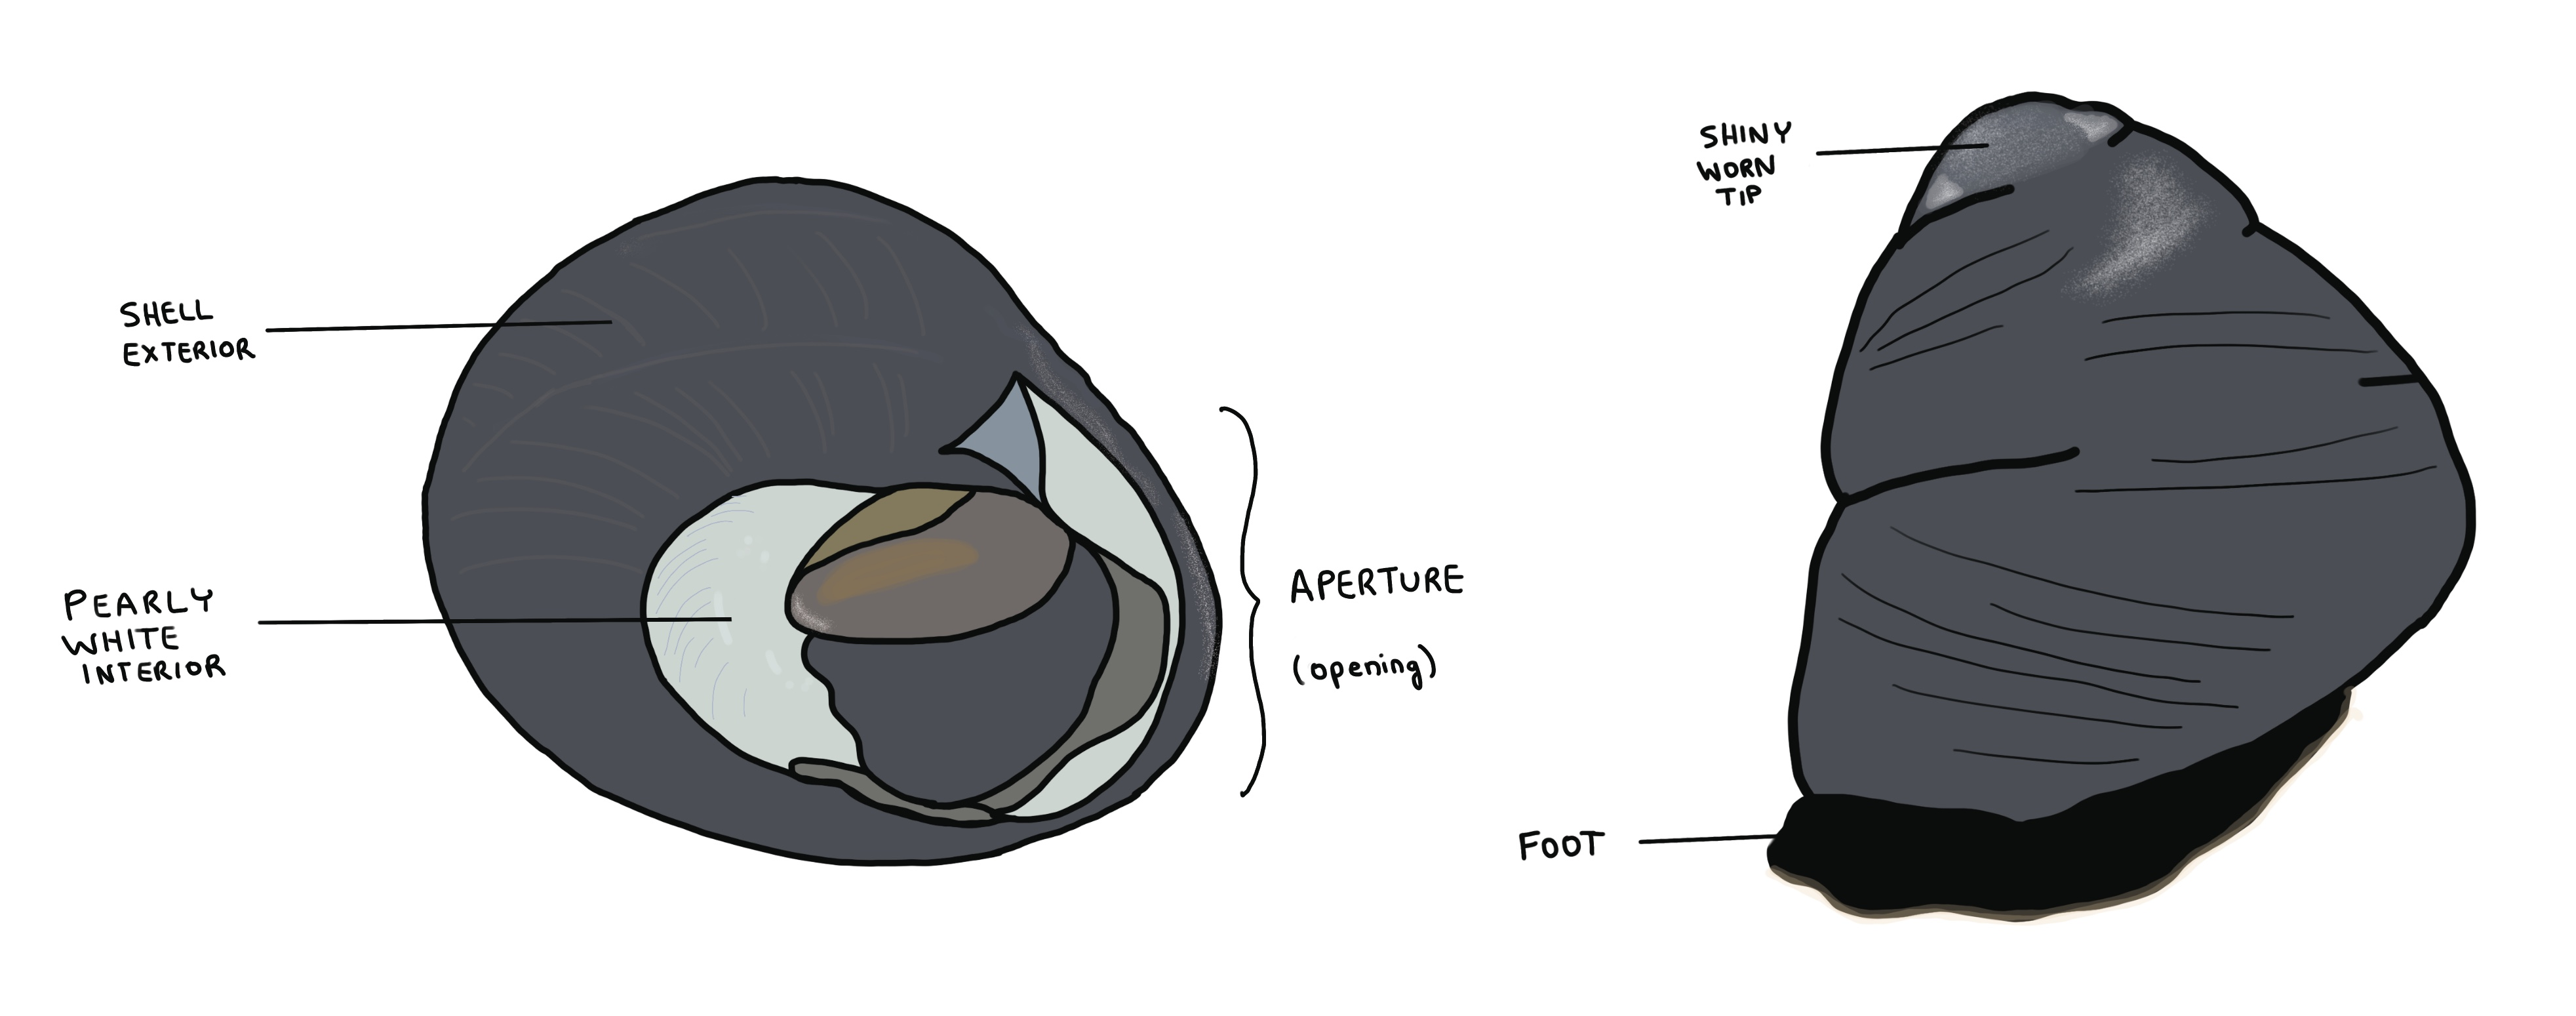
\includegraphics[width=0.5\linewidth,height=0.3\textheight]{/Users/mer/Github/species-id-guide-meredithyvr/images/Black Turban Drawings} \hfill{}

\caption{A drawn diagram of *Tegula funebralis*. The left drawing shows the underside of the snail, highlighting the aperture. The right drawing shows an upright view of the snail, including the location of the foot, highlighting the worn tip of the shell.}\label{fig:Black_Turban_Drawing}
\end{figure}

\begin{figure}

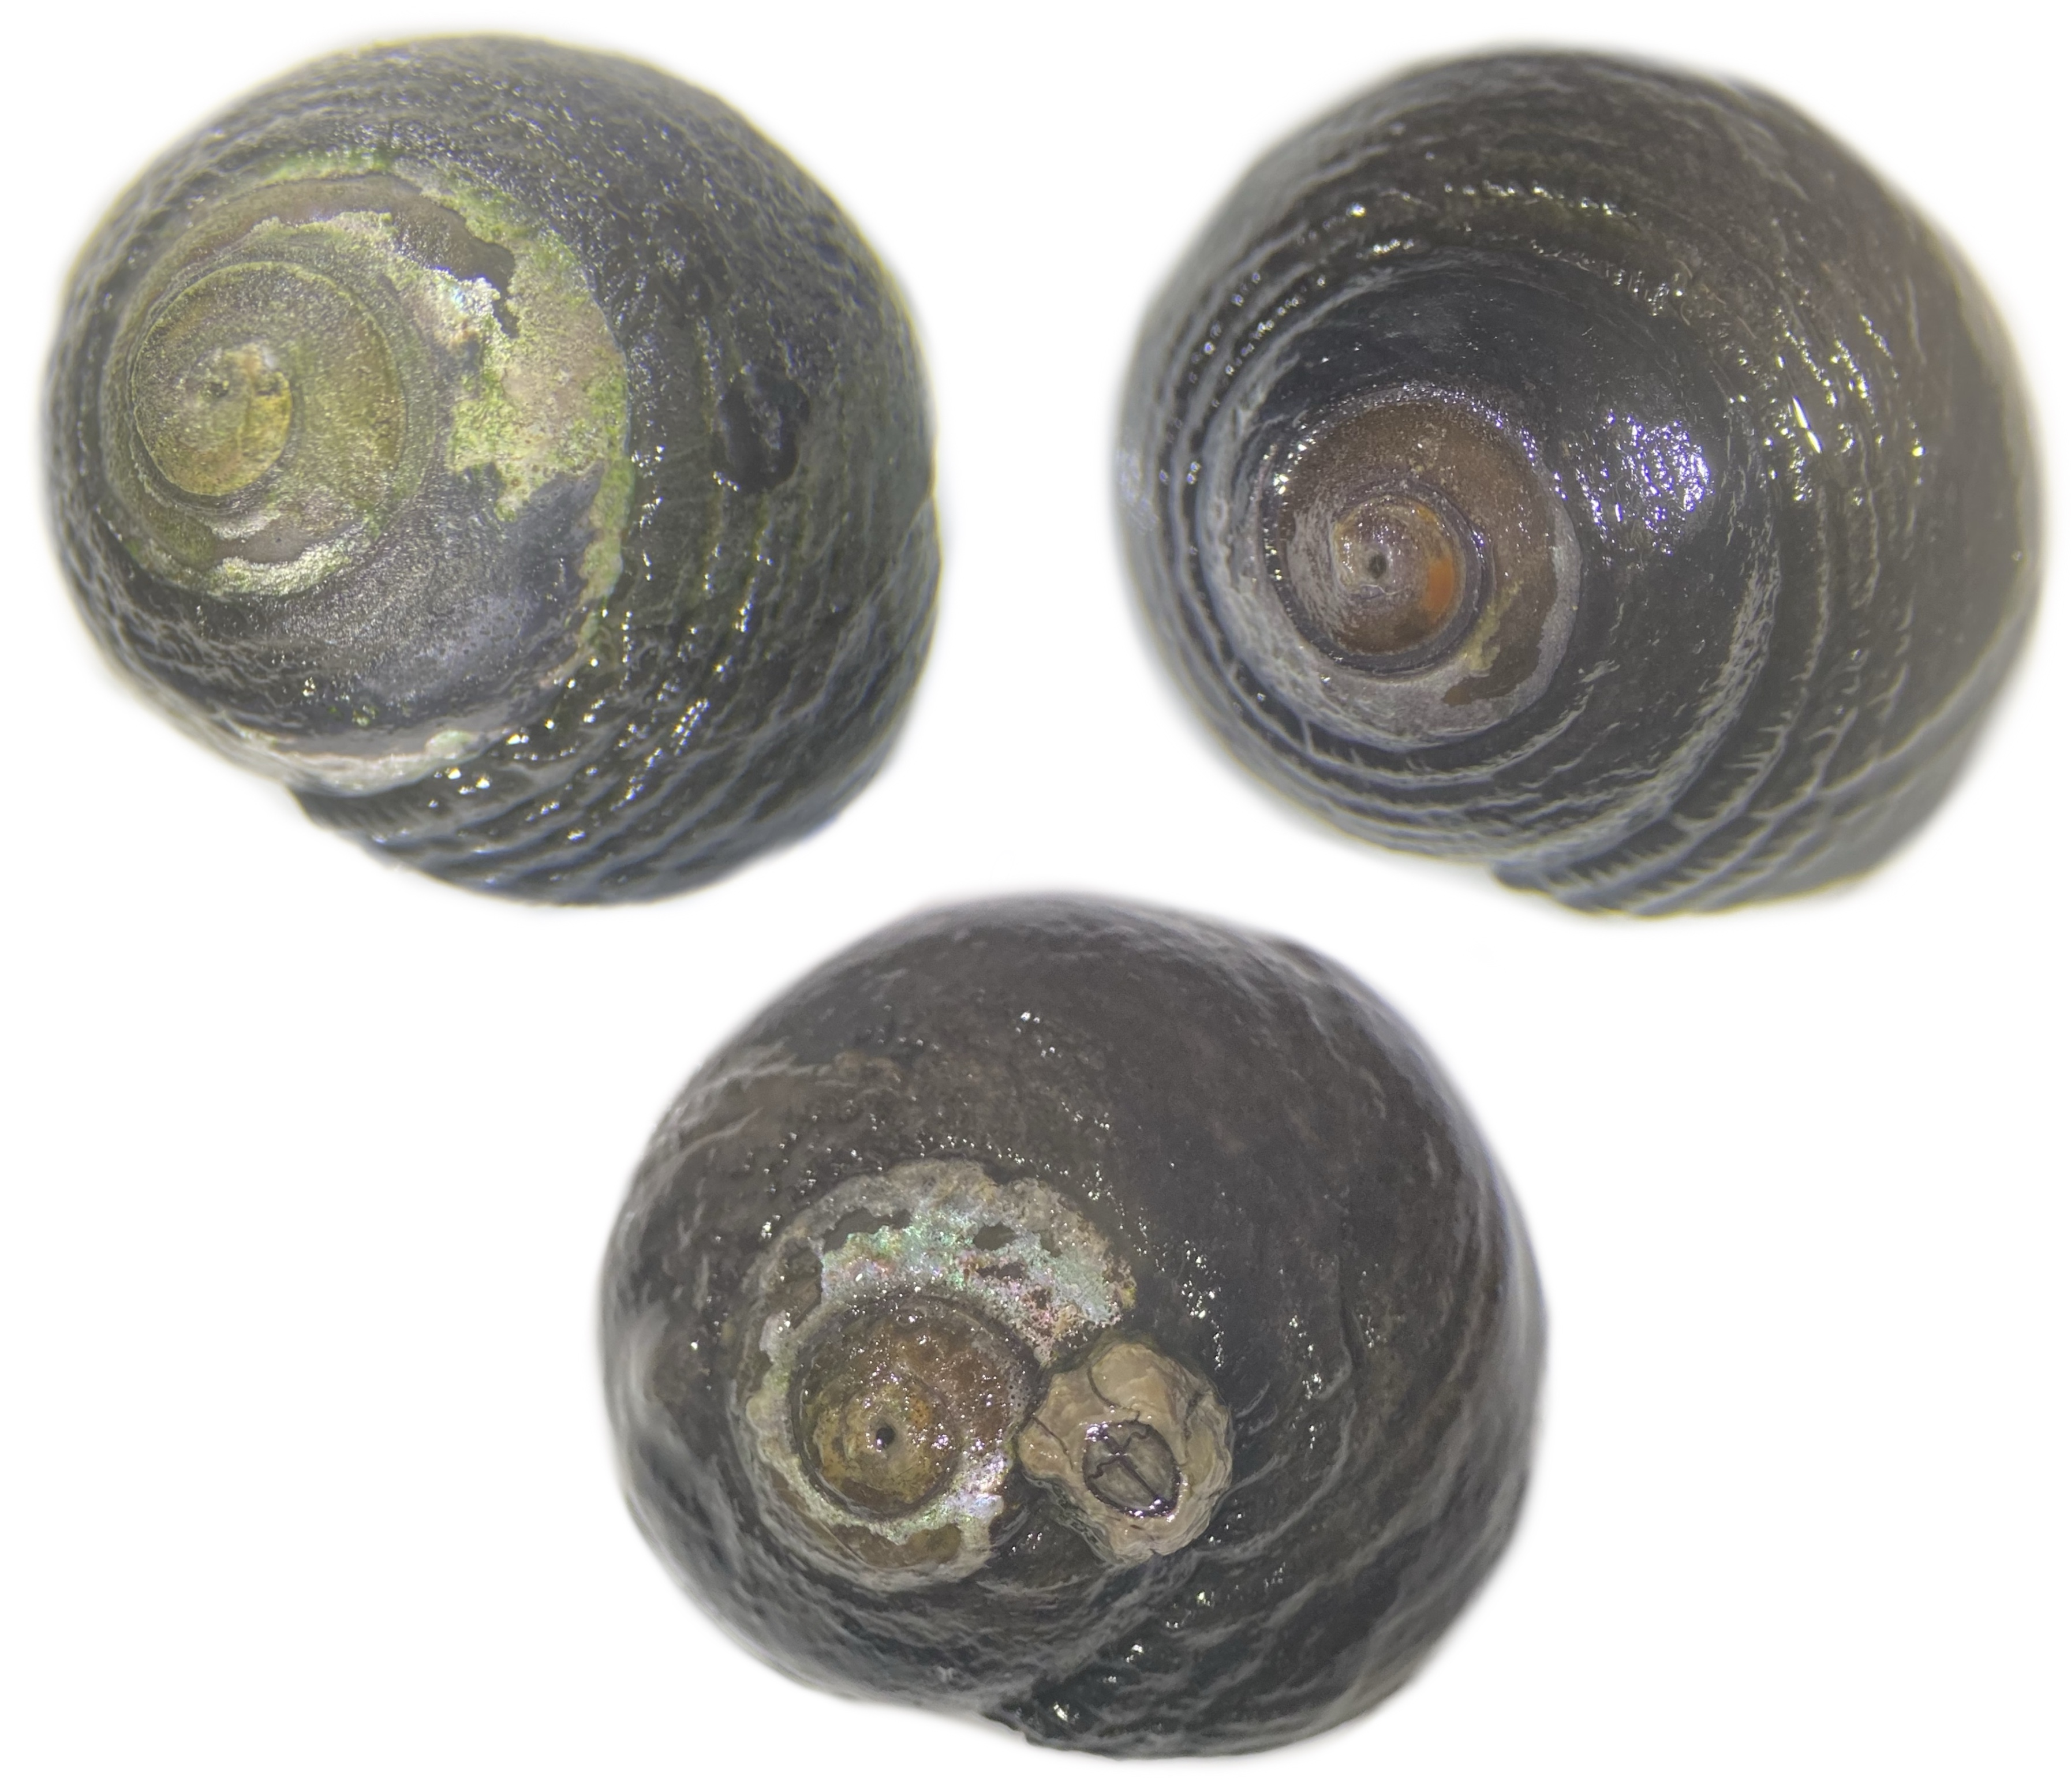
\includegraphics[width=0.5\linewidth,height=0.3\textheight]{/Users/mer/Github/species-id-guide-meredithyvr/images/Black Turban Differences} \hfill{}

\caption{Photos showing three varieties of *Tegula funebralis* snails collected from Scotts Bay in Bamfield, BC on October 15th 2021. This highlights the similarities, such as the variations in tip morphology caused by wear and tear from rough intertidal conditions.}\label{fig:Black_Turban_Differences}
\end{figure}

\newpage

\hypertarget{nucella-ostrina-northern-striped-dogwinkle}{%
\section{\texorpdfstring{\emph{Nucella ostrina} (Northern Striped
Dogwinkle)}{Nucella ostrina (Northern Striped Dogwinkle)}}\label{nucella-ostrina-northern-striped-dogwinkle}}

\hypertarget{description-3}{%
\subsection{Description}\label{description-3}}

This whelk is distinguished by its alternating lines of thick and thin
bands on its shell. Additionally, it can be identified by the three
indistinct whorls on its shell. Colors can range from dark browns,
blacks, and browns to light greys and oranges always with a purple
interior (Meschkat et al., 2014). This snail typically lives in the mid
to high intertidal zones of exposed rocky shorelines from the Bering Sea
to Southern California. The end of its shell known as the umbilicus is
closed. It is most commonly found along barnacle and mussel beds as this
is their preferred diet. This species feeds by drilling a hole with its
radula mouthpart into its prey and extracting digestive enzymes which
are then extracted by its long proboscis (\emph{E-Fauna BC Atlas Page},
2021). \emph{N. ostrina} is commonly mistaken for the northern channeled
dog winkle (\emph{Nucella canaliculata}) as well as the proposed
northern lined dog winkle (\emph{Nucella analoga}). Both of these
species can be distinguished from \emph{N.ostrina} because of their
slender distinctive whorls and smaller body sizes. Mating occurs in
Winter and Spring months with an annual spawn.To reproduce, females
deposit leathery embryonic capsules attached by stalks to the rock from
which the eggs develop and hatch as juveniles after about 2.5-4 months
(Lloyd \& Gosselin, 2007). Therefore, there is no larval feeding stage
and maternal care is critical to the survival of the offspring. Each
capsule will produce about 20 juveniles.

\hypertarget{identification-questions-2}{%
\subsection{Identification Questions}\label{identification-questions-2}}

\begin{enumerate}
\def\labelenumi{\arabic{enumi})}
\item
  Does this snail have a banding pattern that alternates between thick
  and thin stripes?
\item
  Does this snail have three indistinct whorls?
\item
  Is the inside of the shell purple?
\end{enumerate}

\newpage

\hypertarget{figures-3}{%
\subsection{Figures}\label{figures-3}}

\begin{figure}

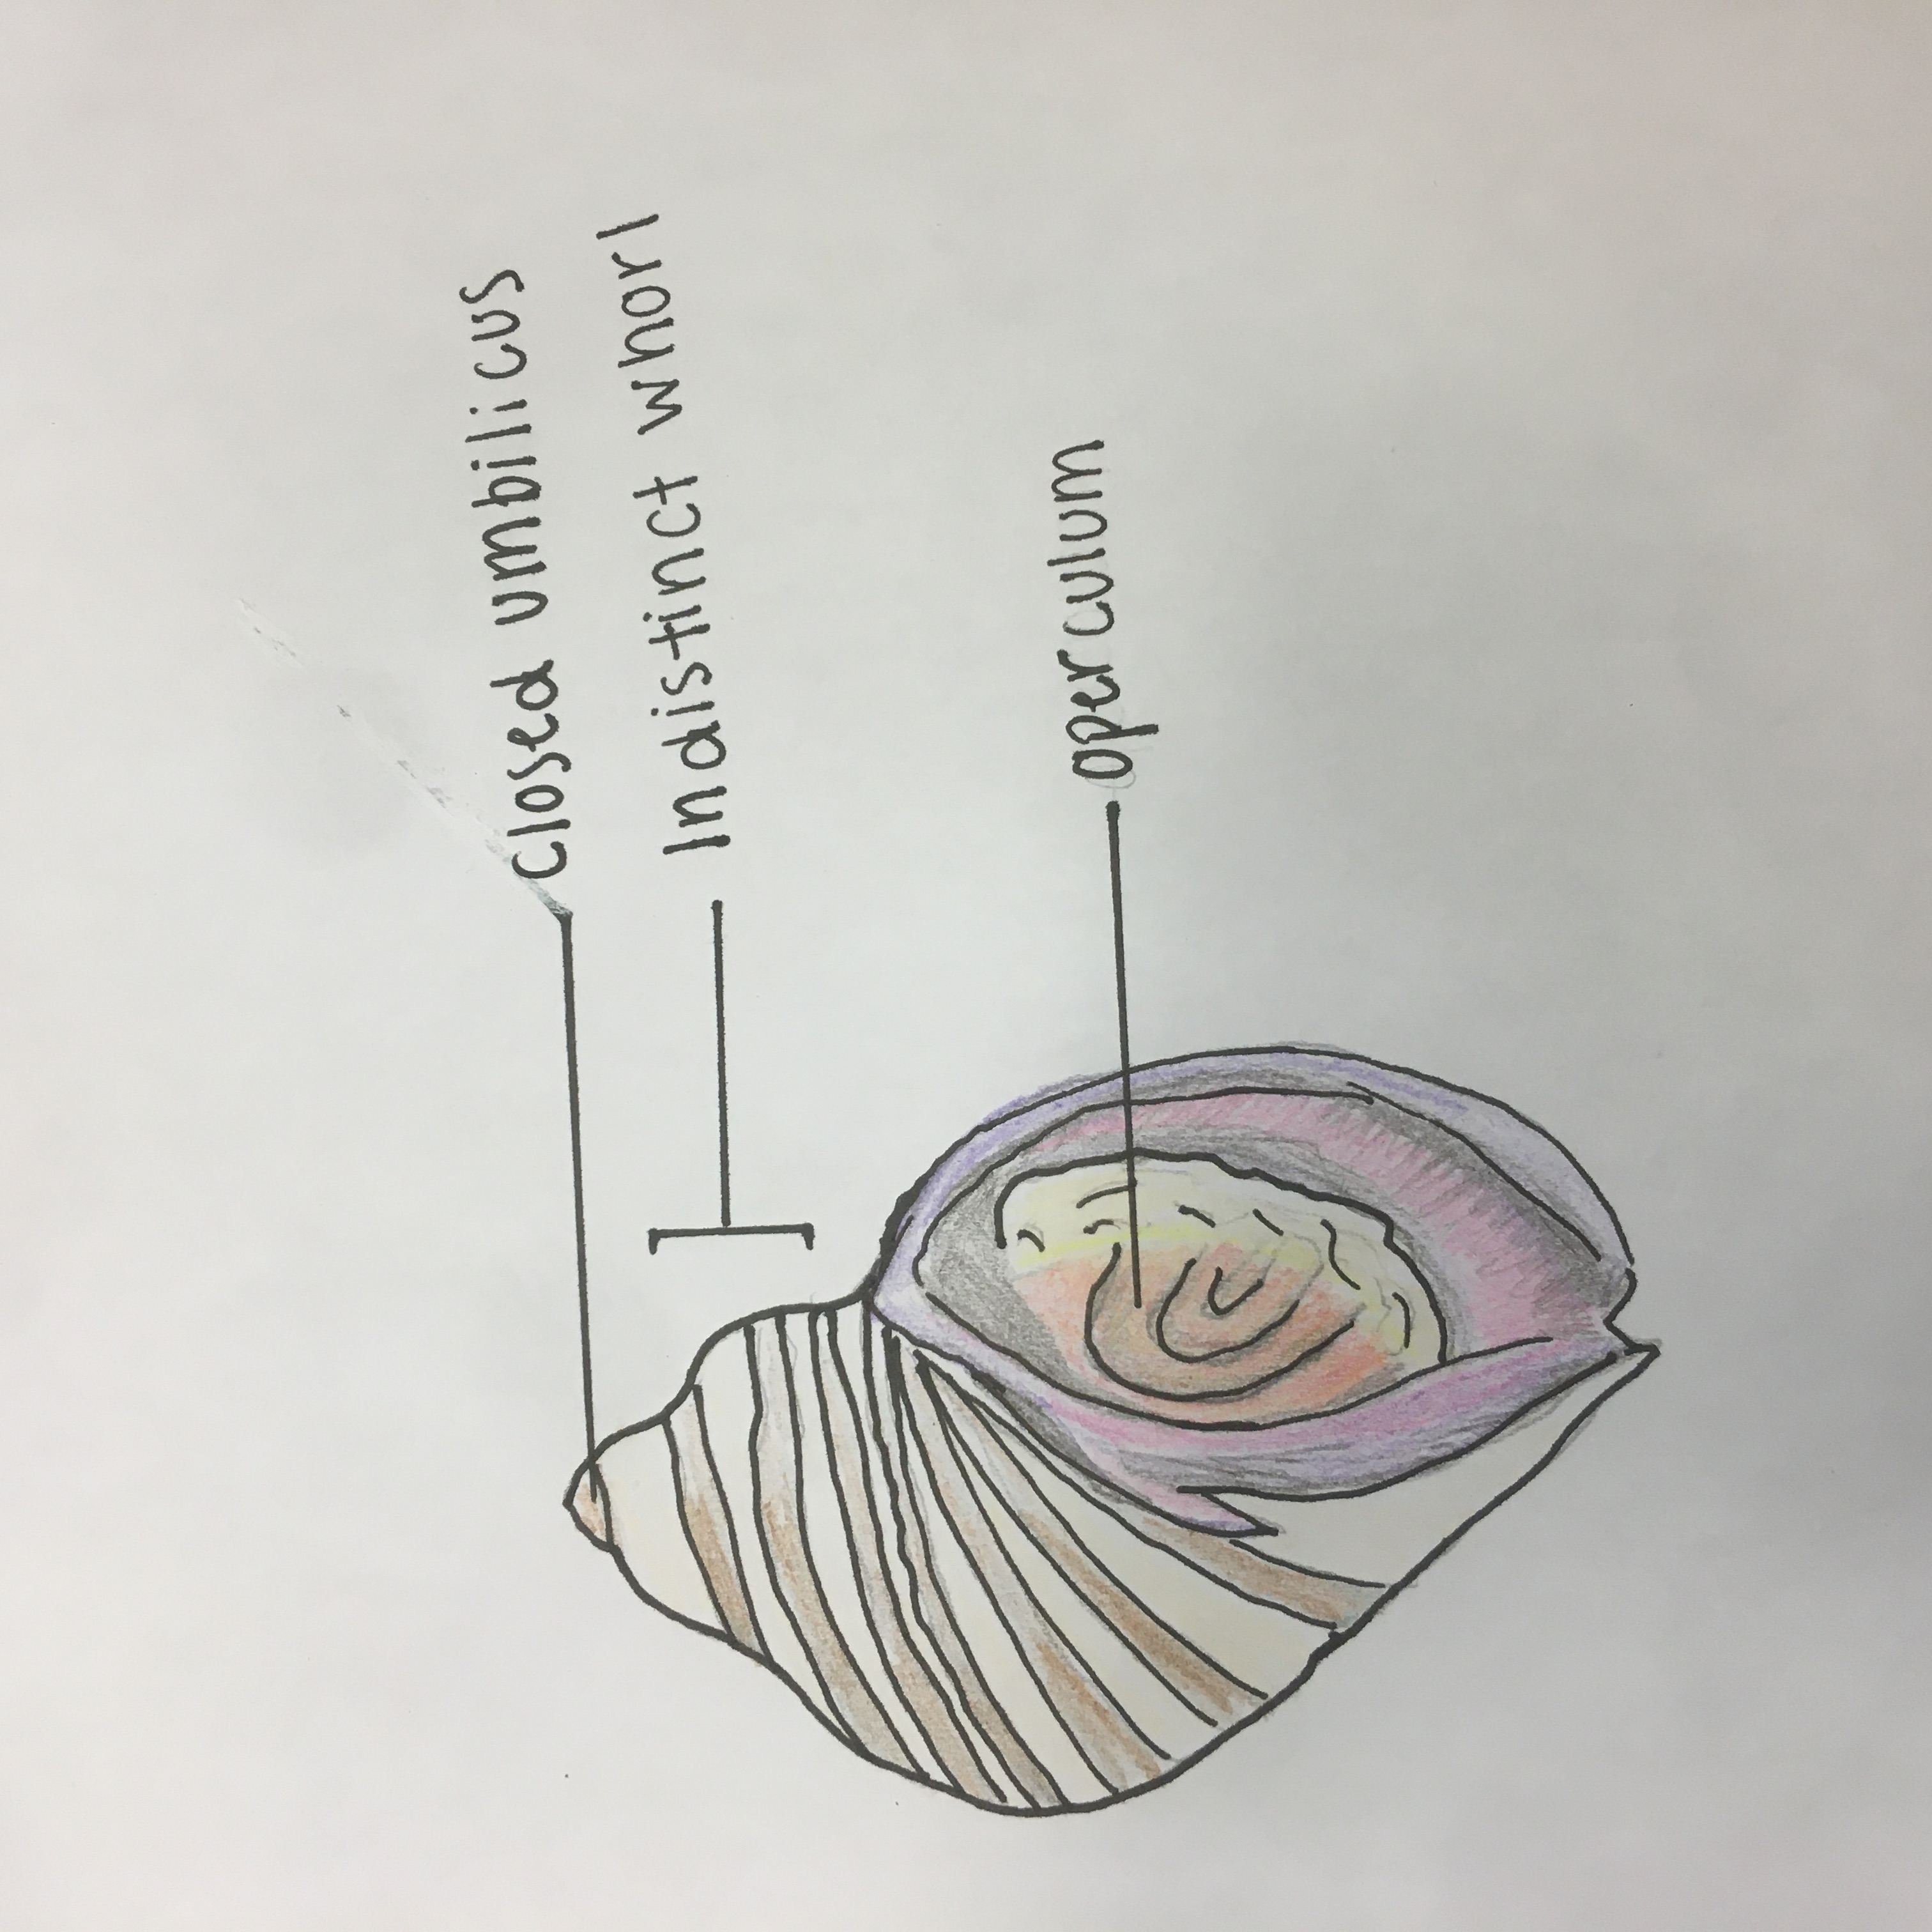
\includegraphics[width=0.5\linewidth,height=0.3\textheight]{/Users/mer/Github/species-id-guide-meredithyvr/images/Northern-Dogwinkle-Drawing} \hfill{}

\caption{Showing *Nucella ostrina* distinctive features such as closed umbilicus, indistinct whorls, purple interior shell and operculum. }\label{fig:Dogwinkle_drawing}
\end{figure}

\begin{figure}

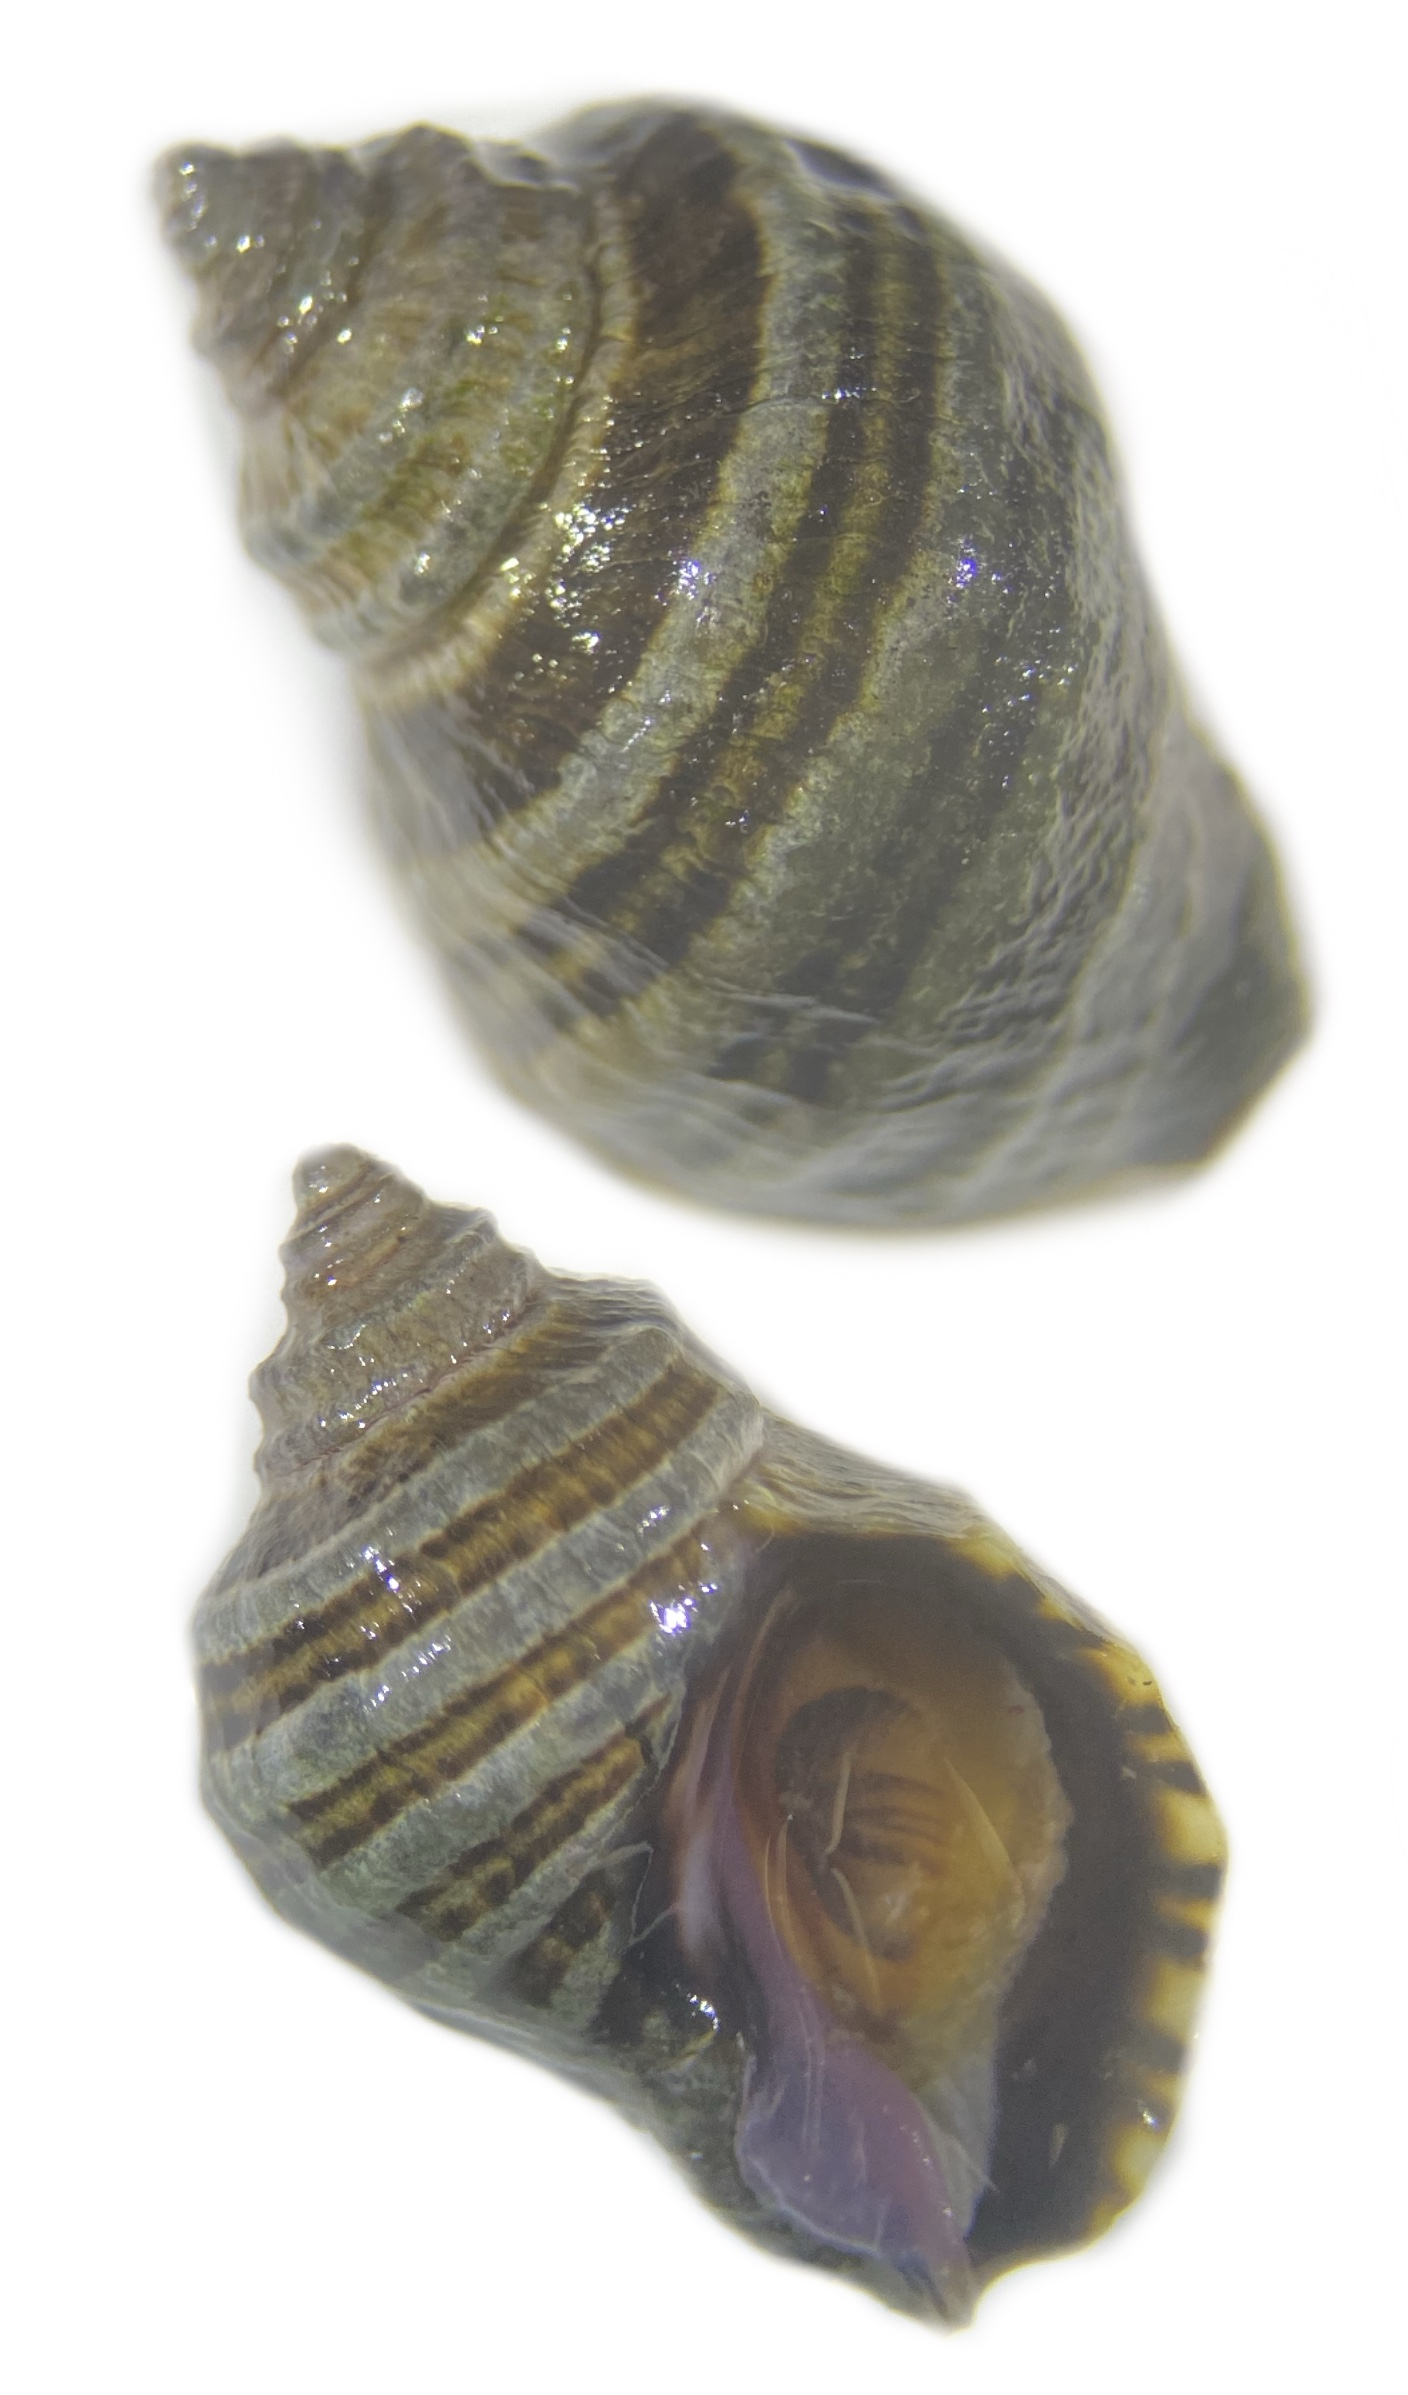
\includegraphics[width=0.5\linewidth,height=0.3\textheight]{/Users/mer/Github/species-id-guide-meredithyvr/images/Northern Striped Dogwinkle Picture} \hfill{}

\caption{Showing *Nucella ostrina* collected from Scotts Bay of Bamfield, BC, Canada in October of 2021.}\label{fig:Dogwinkle_picture}
\end{figure}

\newpage

\hypertarget{supplemental-information}{%
\section{Supplemental Information}\label{supplemental-information}}

\begin{longtable}[]{@{}lrr@{}}
\caption{Shell morphometric measurements of four intertidal
snails}\tabularnewline
\toprule
Species & Length (mm) & Height (mm) \\
\midrule
\endfirsthead
\toprule
Species & Length (mm) & Height (mm) \\
\midrule
\endhead
Nucella\_ostrina & 20.00 & 10.00 \\
Nucella\_lamellosa & 16.00 & 6.30 \\
Nucella\_lamellosa & 19.00 & 9.00 \\
Calliostoma\_ligatum & 5.00 & 4.50 \\
Calliostoma\_ligatum & 10.00 & 12.00 \\
Tegula\_funebralis & 13.10 & 16.80 \\
Tegula\_funebralis & 17.15 & 19.25 \\
Tegula\_funebralis & 18.65 & 19.45 \\
\bottomrule
\end{longtable}

\hypertarget{figures-4}{%
\subsection{Figures}\label{figures-4}}

\begin{figure}
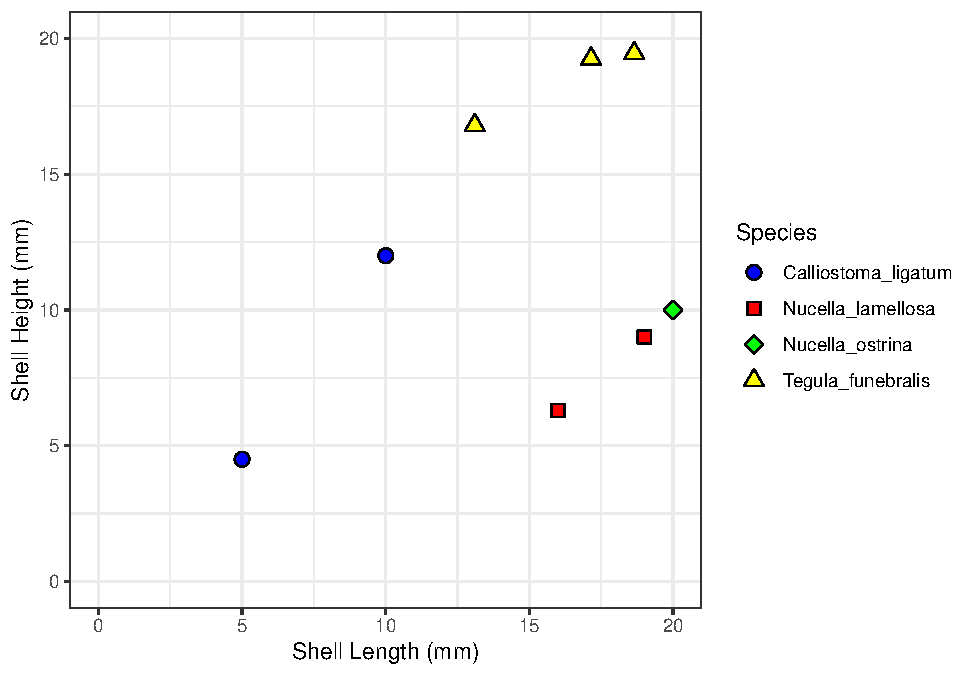
\includegraphics[width=0.8\linewidth,height=0.8\textheight]{Miller_Species_ID_Guide_files/figure-latex/unnamed-chunk-2-1} \caption{Snail shell length and height for four intertidal snails. Snails were collected from Scott's Bay, and measured in lab using calipers}\label{fig:unnamed-chunk-2}
\end{figure}

\newpage

\hypertarget{bibliography}{%
\section{Bibliography}\label{bibliography}}

Bering, N., Hext, T., \& Parker, E. (2017). Nucella lamellosa. In:
Oregon Estuarine Invertebrates: Rudys' Illustrated Guide to Common
Species, 3rd ed.~University of Oregon Libraries and Oregon Institute of
Marine Biology, Charleston, OR.
\url{https://scholarsbank.uoregon.edu/xmlui/bitstream/handle/1794/12913/N_lamellosa_2017_final.pdf?sequence=3}

Carefoot, T. (2021) Nucella lamellosa (Gmelin, 1791) Dog Whelk; Frilled
Dogwinkle; Wrinkled Dog Wheld. E- Fauna BC: Electronic Atlas of the
Wildlife of British Columbia.
\url{http://linnet.geog.ubc.ca/efauna/Atlas/Atlas.aspx?sciname=Nucella\%20lamellosa\&ilifeform=184}

Crowles, D. (2004). Calliostoma ligatum. Invertebrates of the Salish
Sea. Walla Walla University.
\url{https://inverts.wallawalla.edu/Mollusca/Gastropoda/Prosobranchia/Order_Archaegastropoda/Suborder_Trochina/Trochidae/Calliostoma_ligatum.html}

E-Fauna BC Atlas Page. (2021). \emph{E-Fauna BC. Nucella ostrina}
(Gould, 1852) Dog Whelk; Dog Winkle.
\url{http://linnet.geog.ubc.ca/efauna/Atlas/Atlas.aspx?sciname=Nucella\%20ostrina}

Erlandson, J. M., Ainis, A. F., Braje, T. J., Jew, N. P., McVey, M.,
Rick, T. C., Vellanoweth, R. L., \& Watts, J. (2015). 12,000 Years of
Human Predation on Black Turban Snails (Chlorostoma funebralis) on Alta
California's Northern Channel Islands. California Archaeology, 7(1),
59--91. \url{https://doi.org/10.1179/1947461X15Z.00000000056}

Fretwell, K., \& Starzomski, B. (2013). \emph{Black turban snail, Tegula
funebralis. Biodiversity of the Central Coast}.
\url{https://www.centralcoastbiodiversity.org/black-turban-snail-bull-tegula-funebralis.html}

Harbo, R. M. (2011). Whelks to Whales: Coastal Marine Life of the
Pacific Northwest (Revised Second ed.). Harbour Publishing. Turban
Snails, Topsnails, 131.

Harbo, R. M. (2011). Whelks to Whales: Coastal Marine Life of the
Pacific Northwest (Revised Second ed.). Harbour Publishing, BC. Whelks,
Dogwinkles: 144-145.

Hiebert, T. C., Butler, B. A., \& Shanks, A. L. (1979). Tegula
funebralis in Oregon Estuarine Invertebrates: Rudys' Illustrated Guide
to 140 Common Species (No.~3). University of Oregon Libraries and Oregon
Institute of Marine Biology.
\url{https://oimb.uoregon.edu/wp-content/uploads/2019/03/T_funebralis_2018.pdf}

Hoffman, D. L. (1980). Defensive Responses of Marine Gastropods
(Prosobranchia, Trochidae) to Certain Predatory Seastars and the Dire
Whelk, Searlesia dira (Reeve). Pacific Science, 34(3), 233-243.

Holyoak, A.R. (1988). Spawning and larval development of the trochid
gastropod Calliostoma ligatum. The Veliger, 30(4), 369-371

Lloyd, M. J., \& Gosselin, L. A. (2007). Role of Maternal Provisioning
in Controlling Interpopulation Variation in Hatching Size in the Marine
Snail Nucella ostrina. The Biological Bulletin, 213(3), 316--324.
\url{https://doi.org/10.2307/25066649}

Meschkat, C., Fretwell, K., \& Brian Starzomski, B. (2014).
\emph{Northern striped dogwinkle • Nucella ostrina. Biodiversity of the
Central Coast}.
\url{https://www.centralcoastbiodiversity.org/northern-striped-dogwinkle-bull-nucella-ostrina.html}

Meschkat, C., Fretwell, K., \& Starzomski, B. (2013). \emph{Blue
topsnail, Western ridged top shell. Calliostoma ligatum. Biodiversity of
the Central Coast}.
\url{https://www.centralcoastbiodiversity.org/blue-topsnail-bull-calliostoma-ligatum.html}

Proudfoot, B, \& Fretwell, K. (2015). \emph{Frilled Dogwinkle, Wrinkled
Dogwinkle • Nucella Lamellosa. Biodiversity of the Central Coast}.
\url{https://www.centralcoastbiodiversity.org/frilled-dogwinkle-bull-nucella-lamellosa.html}.

Tuskes, P. M. (2019). Calliostomatidae of the northeast Pacific.
Zoosymposia, 13, 83-96.
\url{http://dx.doi.org/10.11646/zoosymposia.13.1.9}

\end{document}
